\documentclass{beamer}   % [notes=show,handout]

\usepackage{tikz}
\usepackage{graphicx}
\usepackage{hyperref}
\mode<presentation>

\usetheme{Frankfurt}%
\usecolortheme{seagull}

\definecolor{garnet}{RGB}{136,0,0}
% \definecolor{clarksonGreen}{RGB}{0,71,28}
\definecolor{clarksonGreen}{RGB}{0,52,21}
\setbeamercolor{palette primary}{fg=clarksonGreen,bg=white}
\setbeamercolor{palette secondary}{fg=clarksonGreen,bg=white}
\setbeamercolor{palette tertiary}{fg=clarksonGreen,bg=white}
\setbeamercolor{palette quaternary}{bg=clarksonGreen,fg=white}
\setbeamercolor{block title}{fg=black,bg=black!15}
\setbeamercolor{block body}{fg=black,bg=black!10}
\setbeamercolor{titlelike}{bg=clarksonGreen,fg=white} % parent=palette quaternary}


\setbeamertemplate{footline}{\hspace*{.5cm}\scriptsize{\insertauthor
    \hspace*{50pt} \hfill\insertframenumber\text{/}\inserttotalframenumber\hspace*{.5cm}}}

\newcommand{\R}{\mathbb{R}}
\newcommand{\lp}{\left(}
\newcommand{\rp}{\right)}
\newcommand{\half}{\frac{1}{2}}
\newcommand{\pderiv}[1]{\frac{\partial}{\partial {#1}}}
\newcommand{\mderiv}[2]{\frac{\partial^{#1}}{\partial^{#1} {#2}}}
\begin{document}



\part{Introduction}
\lecture{Introduction}{Introduction}


\title{Fund Management for Automobile and Deer Collisions}
\subtitle{Actuarial Considerations}

\author{Kelly Black, Candace Liu, Elizabeth Sweeney, Lindong Zhou}
\institute{Clarkson University, The College of New Jersey, and
  Middlebury College} 
\date{18 October, 2013}

\begin{frame}[plain]
  \titlepage
\end{frame}

\begin{frame}
  \frametitle{Outline}
  \vspace{-5mm}
  \tableofcontents[]
\end{frame}

\section{Introduction}

\begin{frame}
  \begin{center}
    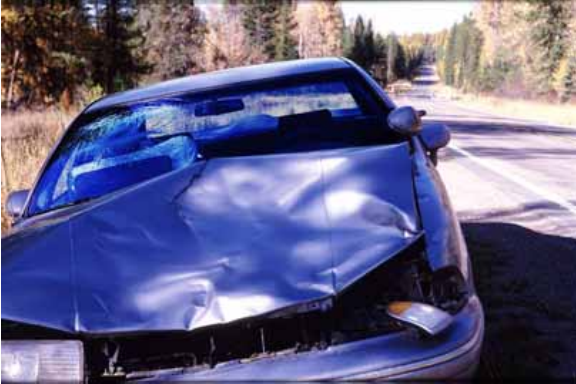
\includegraphics[height=5cm]{propertyCongressionalStudy}
  \end{center}
  From the Wildlife-Vehicle Collision Reduction Study, a report to the
  US Congress, 2008.
\end{frame}

\begin{frame}
  \frametitle{The Problem}

  From the Wildlife-Vehicle Collision Reduction Study, a report to the
  US Congress, 2008.
  \begin{itemize}
  \item Estimated 300,000 collisions per year between wildlife and
    vehicles.
  \item Events that result in less that \$1,000 in property damage
    tend not to be reported.
  \item From 1990 to 2004, total number of motor vehicle crashes has
    had little change, but yearly rate of collisions with wildlife
    increased by about 50\%. (Roughly 5\% of all accidents by 2004.)
  \end{itemize}
  % http://trid.trb.org/view.aspx?id=884083
  
\end{frame}

\begin{frame}
  \frametitle{The Problem}

  Romin \& Bissonette, 1996 (Wildlife Society Bulletin), a survey of
  41 states:
  \begin{itemize}
  \item 120 people killed in accidents
  \item A variety of mitigation strategies
    \begin{itemize}
    \item Signs (lighted and passive) % consensus that this does not work. 
    \item Reflectors
    \item Lighting
    \item Fencing 
    \item Vegetation
    \item Right of ways, underpasses, and overpasses
      % They *THINK* this is the only one that actually works
    \item Hazing
    \item Reduced speed limits
    \end{itemize}
  \item Not sure what works.
  \item Economic impact is substantial. (Loss of life, Property loss,
    economic loss)
  \end{itemize}
  
  % http://www.jstor.org/stable/3783118
\end{frame}

\begin{frame}
  \frametitle{The Problem}
  
  Sullivan \& Messmer, 2003, (Wildlife Society Bulletin ), viewpoint
  from DOT administrators:
  \begin{itemize}
  \item Difficult to estimate the magnitude of the problem.
  \item 150 people killed in accidents.
  \item Roughly 1.5 million deer-vehicle collisions occurred.
  \item \$1.1  billion in property damages.
  \item Most mitigation strategies either ineffective or untested.
  \item Effectiveness of public awareness campaigns unknown.
  \item Fencing combined with underpasses/overpasses perceived to be
    effective.
  \item Reduced deer population seen as one of the few effective
    solutions.
  \end{itemize}

  % http://www.jstor.org/stable/3784370
\end{frame}

\begin{frame}
  \frametitle{View From the Insurance Industry}
  In the U.S., between July 1, 2011 and June 30, 2012:
  \begin{itemize}
  \item 1.23 million deer-vehicle collisions occurred.
  \item Costs are more than \$4 billion in vehicle damage.
  \item The average claim for deer-vehicle collisions was
    \$3,305 per accident.
  \item The Insurance Institute for Highway Safety (IIHS) noted
    that deer-vehicle collisions in the U.S. cause about 200
    fatalities annually.
  \end{itemize}
  \emph{(State Farm, Insurance Journal)}
\end{frame}

\begin{frame}
  \frametitle{Mitigation}
  
  \begin{itemize}
  \item Schwabe \textit{et al}, has examined numerous strategies
    for mitigating the risks.
    % http://www.jstor.org/stable/3784524
  \item Malo, \textit{et al}, predict and identify
    problematic locations.
    % http://onlinelibrary.wiley.com/doi/10.1111/j.0021-8901.2004.00929.x/full
  \item Ng, \textit{et al}, identify traffic and environmental factors
    associated with incidents.
    % http://digitalcommons.unl.edu/hwi/79/
  \item Gonser, \textit{et al}, identify spatial variations in deer
    vehicle collisions.
    % http://www.sciencedirect.com/science/article/pii/S0143622808000817
  \end{itemize}

\end{frame}

\begin{frame}
  \frametitle{Insurance Issues}
  We look at one county in Ohio, Athens County, Ohio.
  \begin{itemize}
  \item 1999 Gramm-Leach-Bliley Financial Services Modernization Act
    gives each state the power to monitor the financial health and
    practices of insurance companies.
    % http://www.ohioinsurance.org/factbook/2003-04/chapter7/chapter7_f.shtml
  \item Ohio requires that insurance balance be kept in low risk
    funds.
  \item This area studied by Schwabe.
  \end{itemize}
\end{frame}

\section{Population Biology}

\begin{frame}
  \frametitle{Deterministic View}

  We assume that there are low predation rates, and interactions with
  people represent the greatest threats to white-tailed deer.
  \begin{eqnarray*}
    \frac{d}{dt} x & = & r x \lp 1 - \frac{x}{L} \rp - h x.
  \end{eqnarray*}

  Combining terms, the equation can be rewritten as
  \begin{eqnarray*}
    \frac{d}{dt} x & = & \tilde{r} x \lp 1 - \frac{x}{\tilde{L}} \rp,
  \end{eqnarray*}
  where
  \begin{eqnarray*}
    \tilde{r} & = & r-h, \\
    \tilde{L} & = & \frac{r-h}{r} L.
  \end{eqnarray*}
  
\end{frame}

\begin{frame}
  \frametitle{Impact of Reducing h}

  Numerous investigators and state agencies have sought to reduce the
  accident rate, $hx$. 

  \vfill

  At equilibrium we have
  \begin{eqnarray*}
    x^* & = & \frac{r-h}{r} L,
  \end{eqnarray*}
  and the accident rate near equilibrium is
  \begin{eqnarray*}
    h x^* & = & h(r-h)\frac{L}{r}.
  \end{eqnarray*}
  
\end{frame}

\begin{frame}
  \frametitle{Impact of Reducing h}
  \centerline{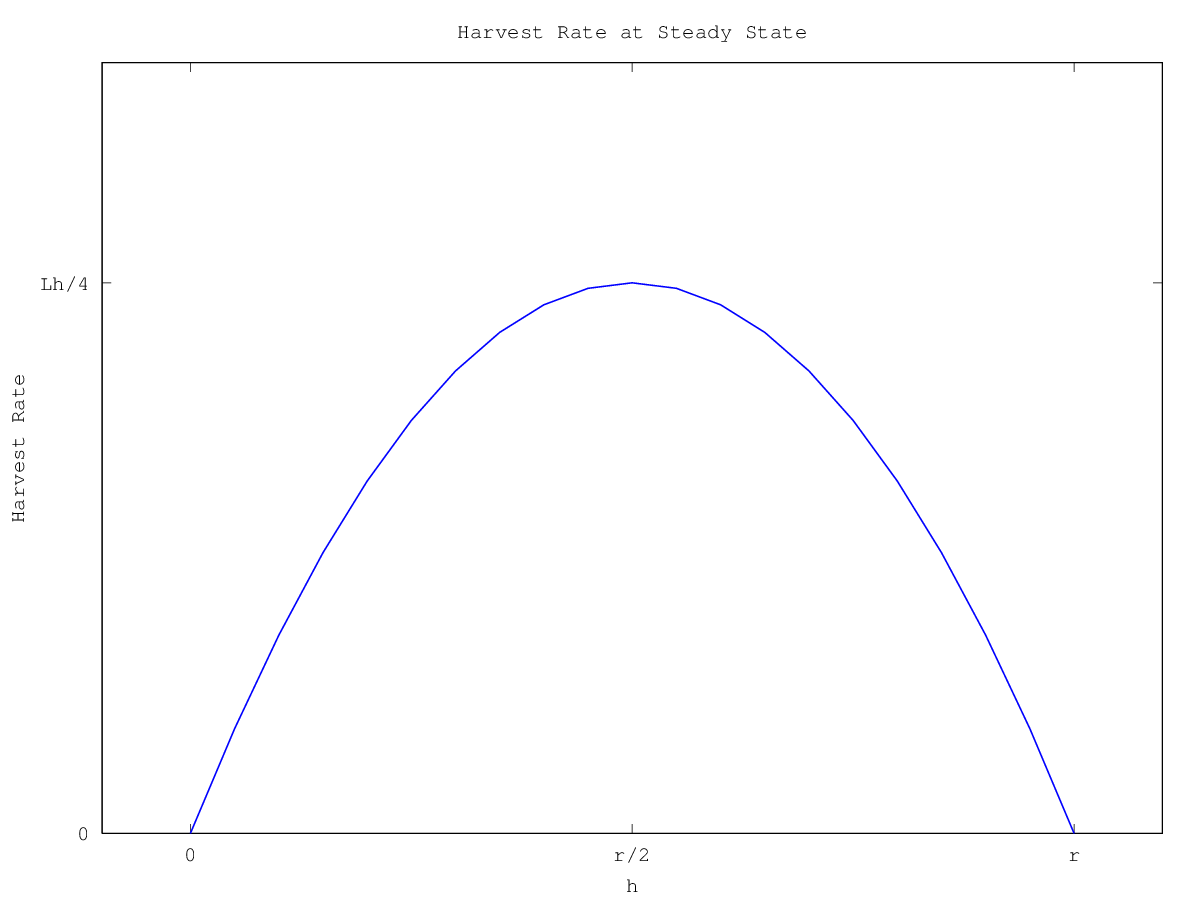
\includegraphics[height=6cm]{reducedHarvest}}
\end{frame}

\begin{frame}
  \frametitle{Impact of Reducing Population}

  Numerous investigators and state agencies have sought to reduce the
  population, $hx$. 

  \vfill

  \begin{eqnarray*}
    \frac{d}{dt} x & = & r x \lp 1 - \frac{x}{L} \rp - h x - Hx.
  \end{eqnarray*}

  \vfill

  At equilibrium we have
  \begin{eqnarray*}
    x^* & = & \frac{r-h-H}{r} L,
  \end{eqnarray*}
  and the accident rate near equilibrium is
  \begin{eqnarray*}
    h x^* & = & h(r-h-H)\frac{L}{r}.
  \end{eqnarray*}


\end{frame}


\begin{frame}
  \frametitle{Impact of Decreasing Population}
  \centerline{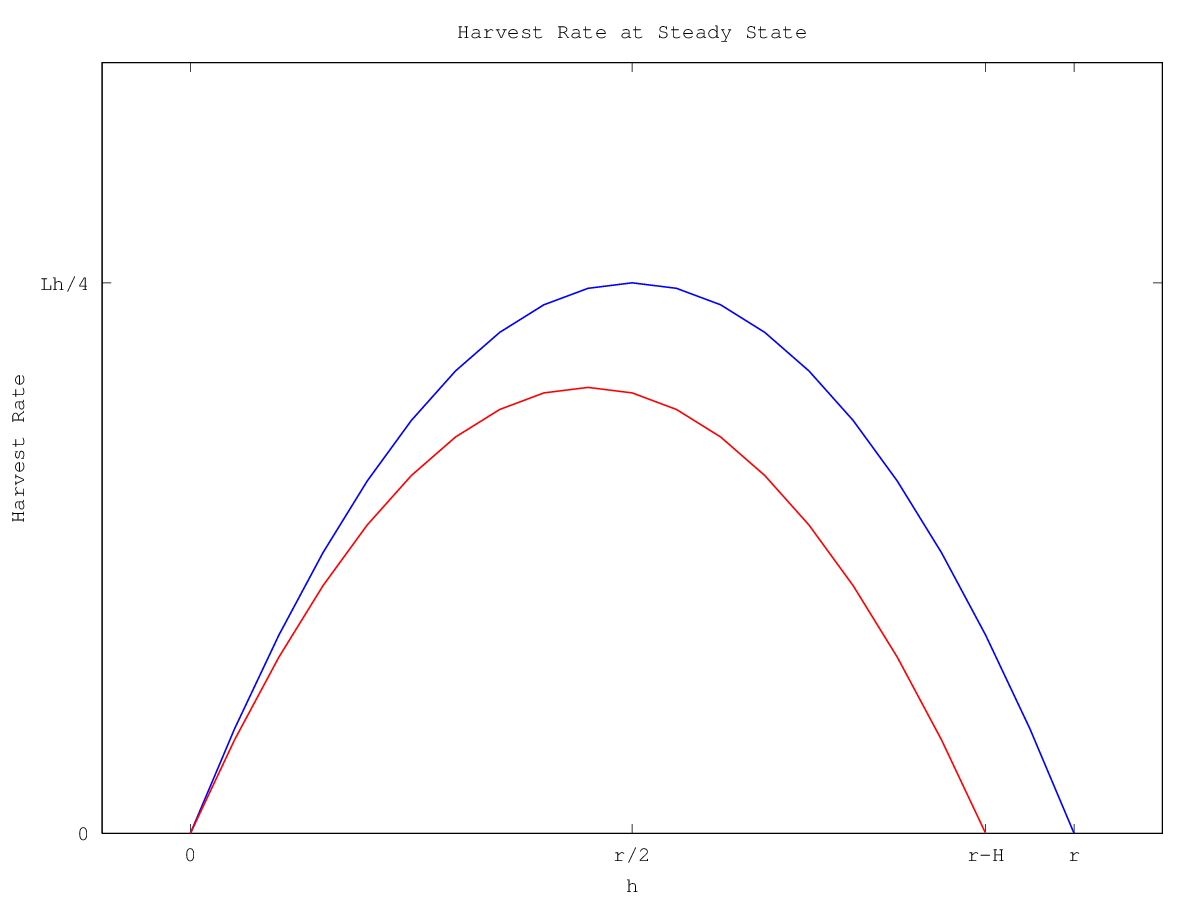
\includegraphics[height=6cm]{reducedPopulation}}
\end{frame}


\begin{frame}
  \frametitle{Dynamic Population Modeling}
  \begin{itemize}
  \item Assumptions
    \begin{itemize}
    \item Population is near carrying capacity.
    \item The only predation is human i.e. hunting and car fatalities.
    \item Migrations rates are balanced across counties.
    \item Customers of one insurance company experience
      the same collision rate as the general population.
    \end{itemize}
  \end{itemize}
\end{frame}


\begin{frame}
  \frametitle{Athens County, Ohio}
  Schwabe, \emph{et al.}, 2000
  \begin{itemize}
  \item Carrying capacity is approximately 28,000
  \item Growth rate is 1.7
  \item Harvest rate is 0.16
  \end{itemize}
\end{frame}


\section{Insurance}

\begin{frame}
  \frametitle{State Regulations and Bond Funds}
  %%%%%%%%%%%%% How insurance companies work
  \begin{itemize}
  \item Low risk government bonds
  \item Premiums from customers
    %%%%% AREA WHERE YOU LIVE AKA DEER, driving record, age, type of car
  \item Claims based on accidents
  \end{itemize}
\end{frame}


\begin{frame}
  \frametitle{Stochastic Modeling}
  \begin{itemize}
  \item Brownian Motion (Random Walks) - $W(t)$
  \item Properties
    \begin{enumerate}[i]
    \item $W(t)$ is continuous
    \item $W(t)$ is nowhere differentiable
    \item If $t_{1}<t_{2}<t_{3}<t_{4}$, \\
      $W(t_{1}), W(t_{2})-W(t_{1}),  W(t_{3})-W(t_{4})$ are independent rando
      m variables
    \item If $0 \le s\le t$ then $W(t)-W(s) \sim N(0, t-s)$
    \end{enumerate}
  \item Gaussian White ``Noise" - $dW$
  \end{itemize}
  %%%%%%%%%% Brownian Motion, Gaussian White Noise
\end{frame}



\begin{frame}
  \frametitle{Models}
  \begin{eqnarray}
    dx &=& \tilde{r} x \lp 1- \frac{x}{\tilde{f}}\rp dt +\alpha x \, dW \\
    dm &=& ( \rho m - \beta x + P) dt - \gamma x \, dW
  \end{eqnarray}
  \begin{itemize}
  \item Known Parameters - $\tilde{r}$, $\tilde{f}$, $\rho$, $\beta$
  \item Unknown Parameters - $\alpha$, $\gamma$, $P$
  \end{itemize}
\end{frame}

\section{Numerics}

\begin{frame}
  \frametitle{Approximation}
  %%%%%%%%% Include figure
  \vspace*{-3em}
  \begin{eqnarray*}
    dX &=& f(X) \, dt + g(X) \, dW \\
  \end{eqnarray*}
  \vspace*{-3em}
  \begin{center}
    $X_{j} =$ approximation of $X(t_{j})$ \\ [20pt]
    % \includegraphics[height=4cm]{approximation}
  \end{center}

\end{frame}



\begin{frame}
  \frametitle{Models}
  \begin{eqnarray*}
    dx &=& \tilde{r} x \lp 1- \frac{x}{\tilde{f}}\rp dt +\alpha x \, dW \\
    dm &=& ( \rho m - \beta x + P) dt - \gamma x \, dW
  \end{eqnarray*}
  \begin{itemize}
  \item Known Parameters - $\tilde{r}$, $\tilde{f}$, $\rho$, $\beta$
  \item Unknown Parameters - $\alpha$, $\gamma$, $P$
  \end{itemize}
\end{frame}

\begin{frame}
  \frametitle{Stochastic Logistic Equation}

  The first equation does not depend on the second:
  \begin{eqnarray*}
    dx &=& \tilde{r} x \lp 1- \frac{x}{\tilde{f}}\rp dt +\alpha x \, dW.
  \end{eqnarray*}

  \vfill

  A solution can be found for the general form (Skiadas, 2010)
  \begin{eqnarray*}
    dx &=& \tilde{r} x \lp 1- \lp\frac{x}{\tilde{f}}\rp^m\rp dt +\alpha x \, dW.
  \end{eqnarray*}
  using the substitution $z=x^{-m}$.

  
\end{frame}

\begin{frame}
  \frametitle{It\^o's Rule (Chain Rule)}

  If $x$ is an It\^o process where (Kuo)
  \begin{eqnarray*}
    x(t) & = & x(0) + \int^t_0 f(s) \, dW(s) + \int^t_0 g(s) \, ds,
  \end{eqnarray*}
  then a function, $\theta(x,t)$, satisfies
  \begin{eqnarray*}
    \theta(x,t) & = & \theta(x(0),0) + 
    \int^t_0 \pderiv{x} \theta(x,s) f(s) \, dW(s) + \\
    & & \int^t_0 \pderiv{t} \theta(x,s) + \pderiv{x} \theta(x,s) g(s) + \half \mderiv{2}{x} \theta(x,s) f^2(s) \, ds
  \end{eqnarray*}

  
\end{frame}

\begin{frame}
  \frametitle{Stochastic Logistic Equation}

  The population equation in integral form
  \begin{eqnarray*}
    x(t) &=& x(0) + \int_0^t \alpha x \, dW(s) + \\
    & & \int_0^t \tilde{r} x \lp 1- \frac{x}{\tilde{f}}\rp dt .
  \end{eqnarray*}

  \vfill

  Here $\theta(x)=x^{-1}$ ($m=1$):
  \begin{eqnarray*}
    \theta(t) &=& \theta(0) + \int^t_0 -c\theta \, dW(s) +
    \int^t_0 \lp -b+1 \rp \theta + b \, ds.
  \end{eqnarray*}


  
\end{frame}


\begin{frame}
  \frametitle{Method of Approximations}
  Milstein Method - $O(\Delta t^{1.5})$
  \begin{eqnarray*}
    X_{j} &=& X_{j-1} + \triangle tf(X_{j-1}) + g(X_{j-1})(W(\tau_{j})-W(\tau_{j-1}
    ))      \nonumber\\ 
    && + \frac{1}{2} g(X_{j-1})g'(X_{j-1})((W(\tau_{j})-W(\tau_{j-1}))^{2}-\triangle t)\\
    j &=& 1,2,... ,L \\
  \end{eqnarray*}
\end{frame}



\begin{frame}
  \frametitle{Parameter Space}
  \hspace*{-1cm}
  %%%%%%%%%% Include 3D plot of parameter space
  % 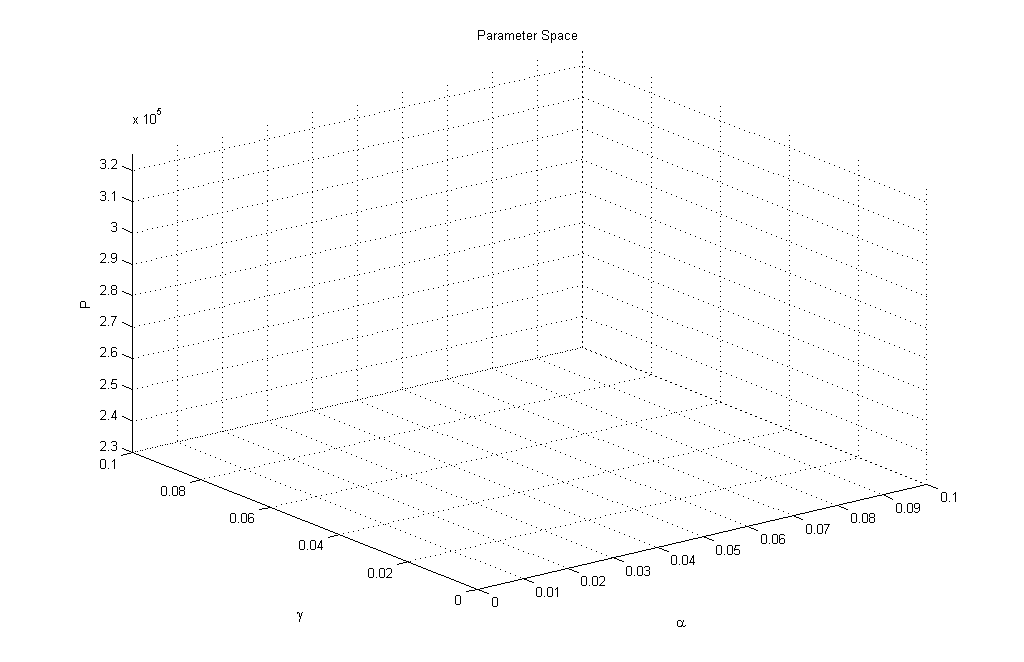
\includegraphics[height=7cm]{parameterspace}
\end{frame}

\begin{frame}
  \frametitle{Parameter Space}
  \hspace*{-1cm}
  %%%%%%%%%% Include 3D plot of parameter space
  % 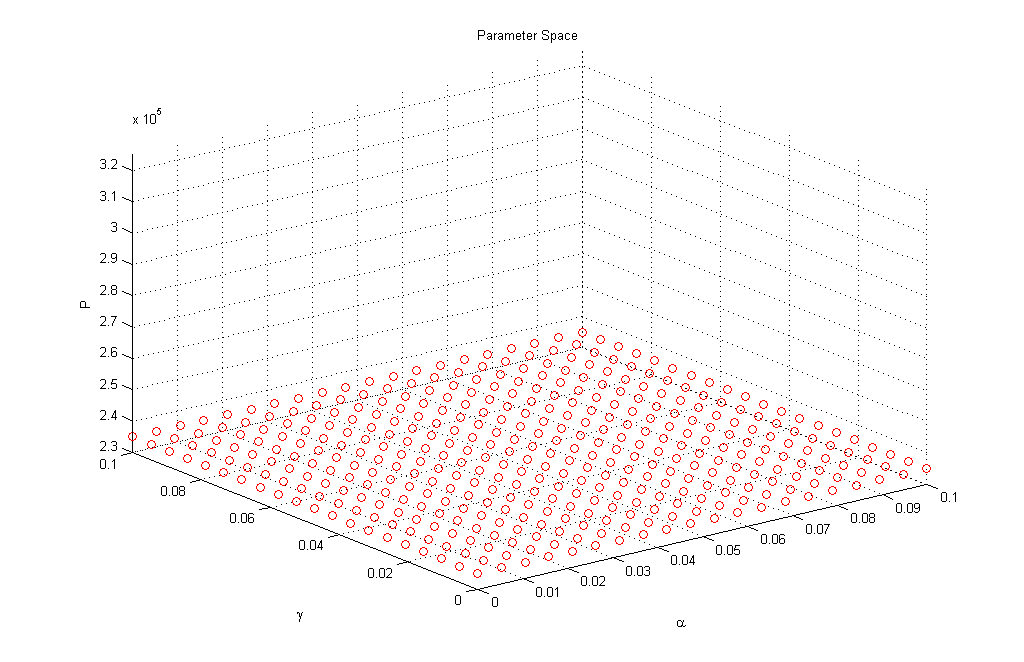
\includegraphics[height=7cm]{parameterspace2}
\end{frame}


\section{Results}

\begin{frame}
  \frametitle{Results - Example for One Run}
  \vspace*{-1cm}
  \begin{eqnarray*}
    \begin{array}{r c l r c l r c l}
      \alpha &=& .05, & \gamma &=& .05, & P &=& 230000
    \end{array}
  \end{eqnarray*}
  \hspace*{-2cm}
  % 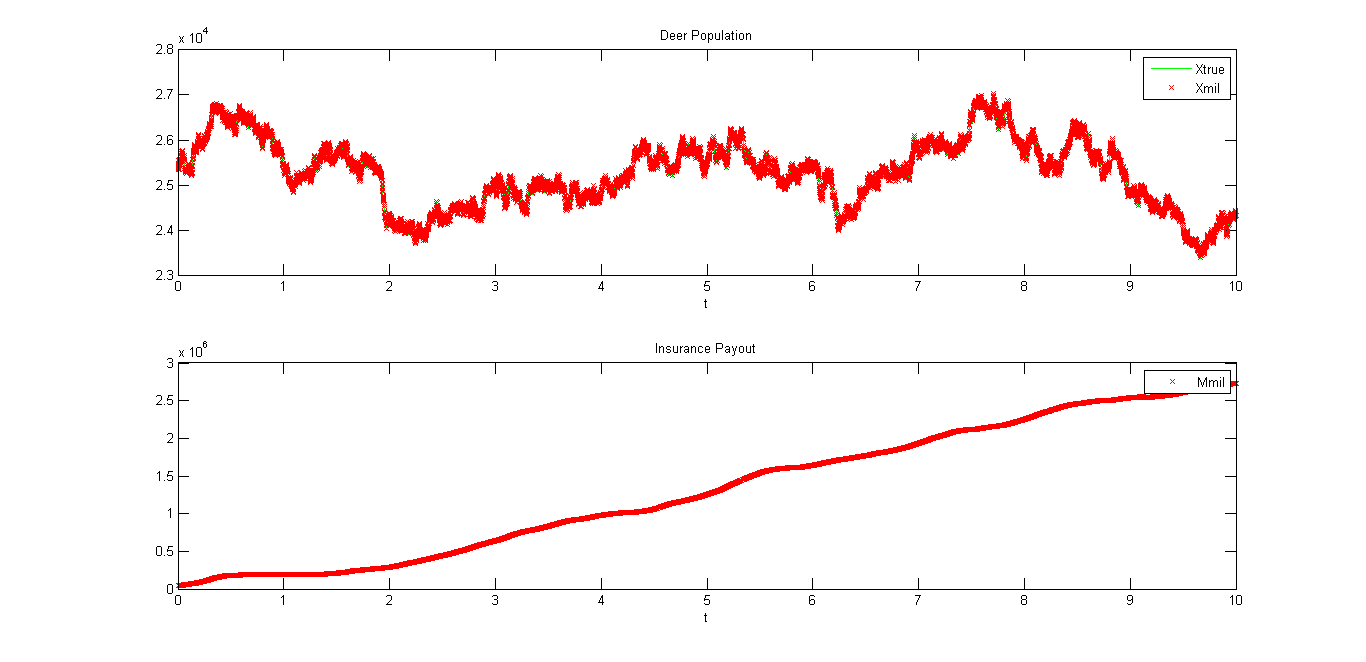
\includegraphics[height=7cm]{deerins}
\end{frame}


\begin{frame}
  \frametitle{Results - X vs. alpha }
  \framesubtitle{500 iterations}
  \hspace*{-5mm}
  % 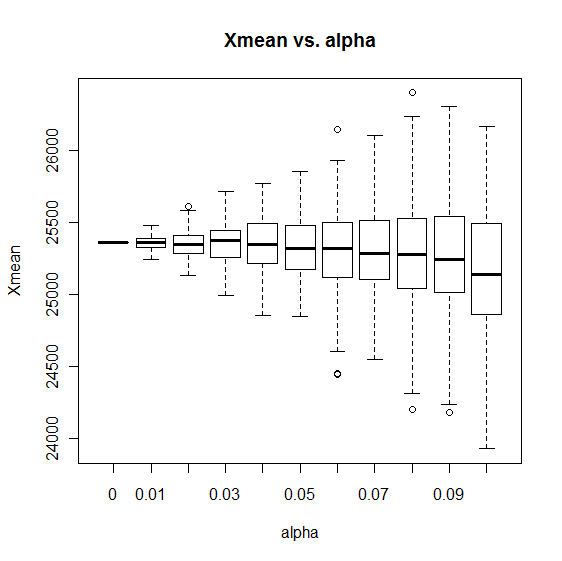
\includegraphics[height=6cm]{boxplot500_xmean_alpha}
  % 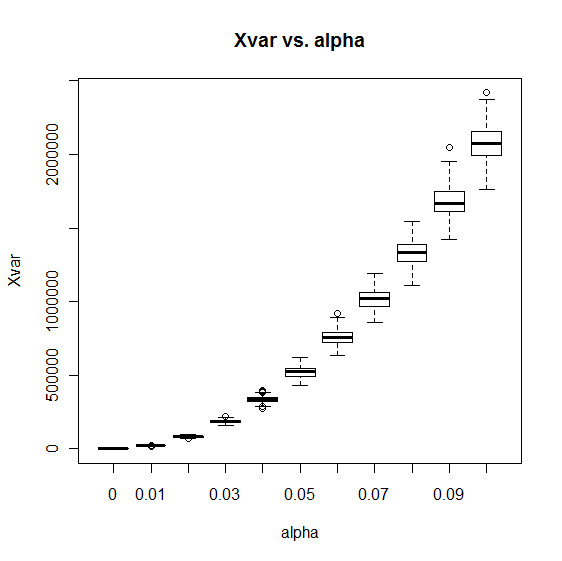
\includegraphics[height=6cm]{boxplot500_xvar_alpha}
\end{frame}

\begin{frame}
  \frametitle{Results - X vs. alpha }
  \framesubtitle{1000 iterations}
  \hspace*{-5mm}
  % 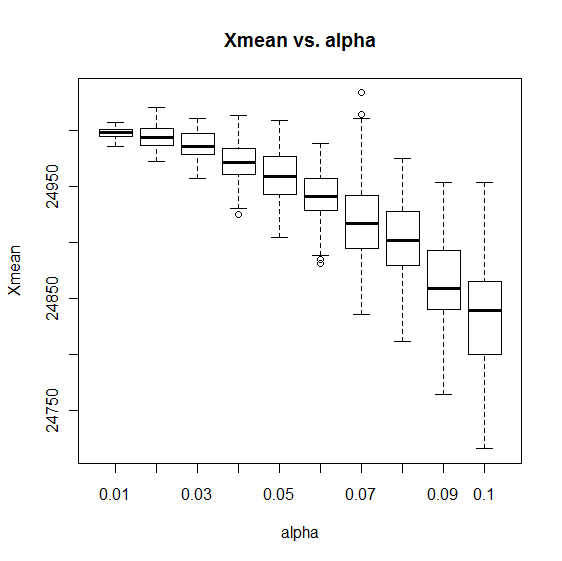
\includegraphics[height=6cm]{boxplot1000_xmean_alpha}
  % 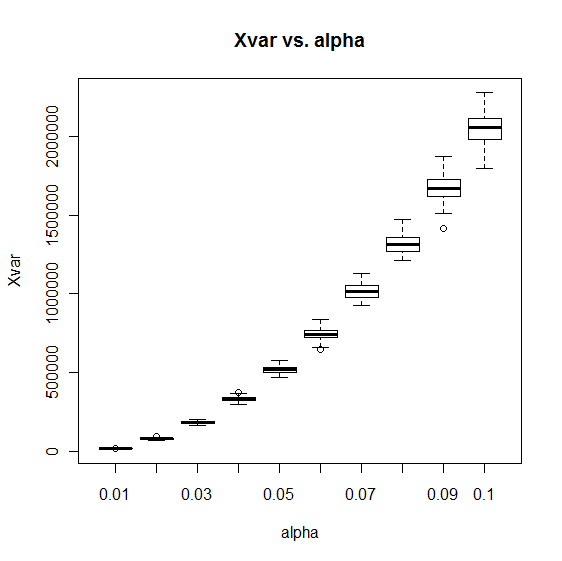
\includegraphics[height=6cm]{boxplot1000_xvar_alpha}
\end{frame}

\begin{frame}
  \frametitle{Results - Histogram}
  \framesubtitle{1000 iterations}
  % 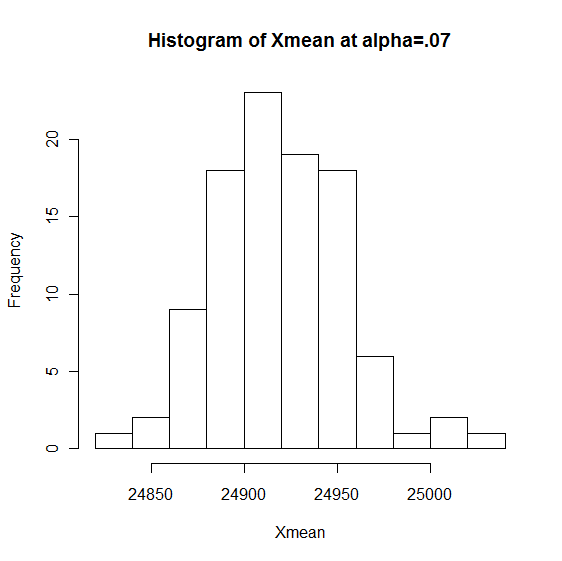
\includegraphics[height=6cm]{hist1000_xmean_alpha07}
\end{frame}



\begin{frame}
  \frametitle{Results - M vs. alpha }
  \framesubtitle{500 iterations}
  \hspace*{-5mm}
  % 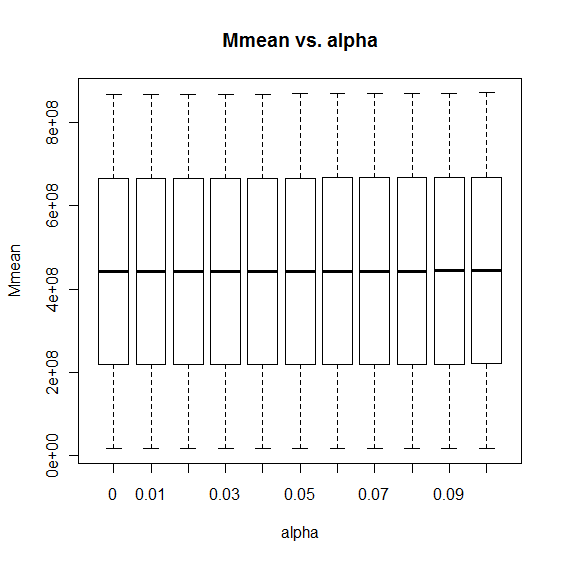
\includegraphics[height=6cm]{boxplot500_mmean_alpha}
  % 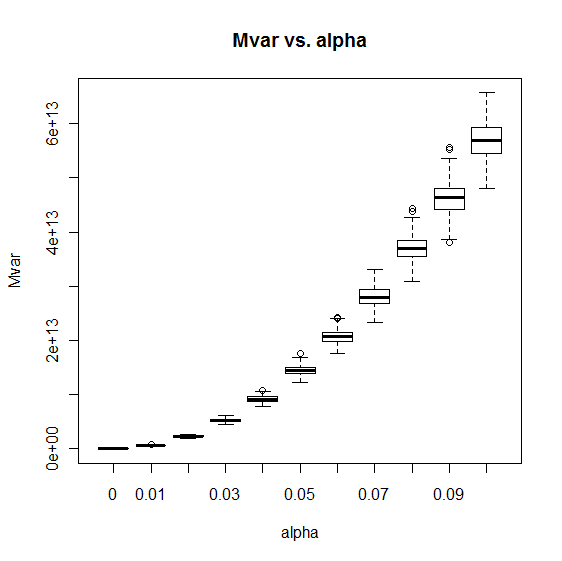
\includegraphics[height=6cm]{boxplot500_mvar_alpha}
\end{frame}

\begin{frame}
  \frametitle{Results - M vs. alpha }
  \framesubtitle{1000 iterations}
  \hspace*{-5mm}
  % 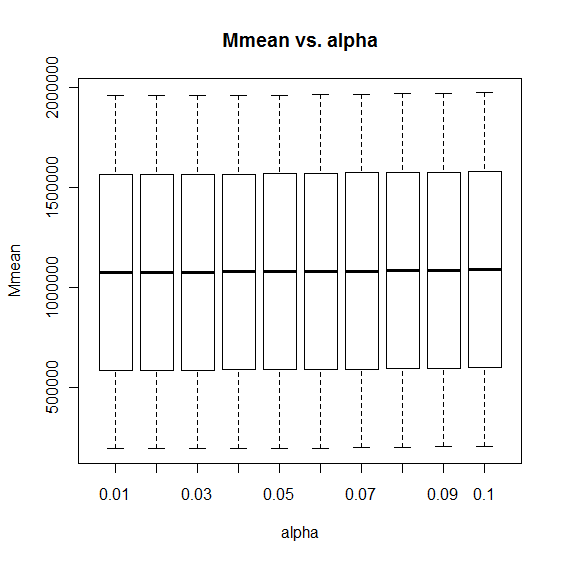
\includegraphics[height=6cm]{boxplot1000_mmean_alpha}
  % 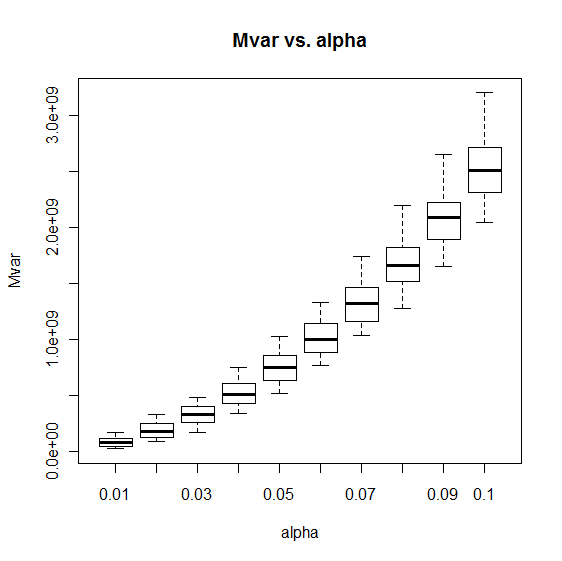
\includegraphics[height=6cm]{boxplot1000_mvar_alpha}
\end{frame}
\begin{frame}
  \frametitle{Results - M vs. gamma }
  \framesubtitle{500 iterations}
  \hspace*{-5mm}
  % 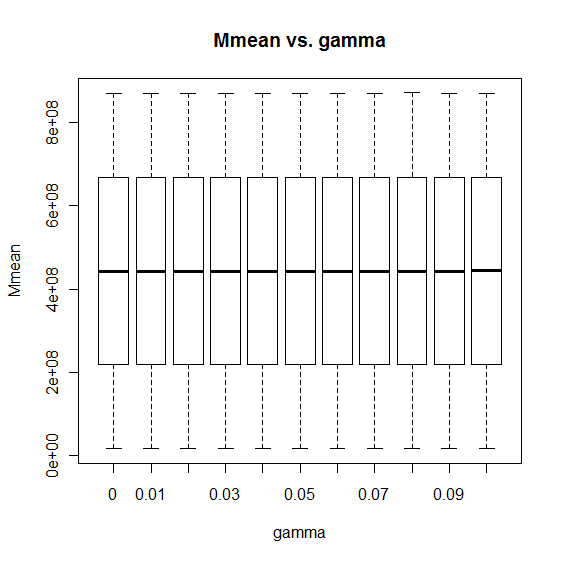
\includegraphics[height=6cm]{boxplot500_mmean_gamma}
  % 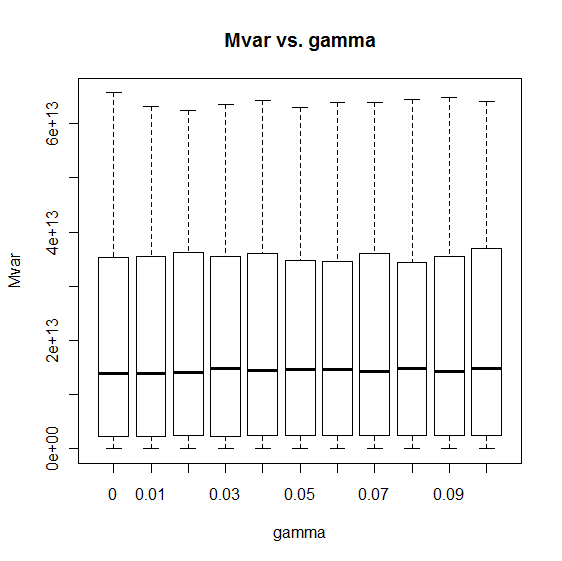
\includegraphics[height=6cm]{boxplot500_mvar_gamma}
\end{frame}

\begin{frame}
  \frametitle{Results - M vs. gamma }
  \framesubtitle{1000 iterations}
  \hspace*{-5mm}
  % 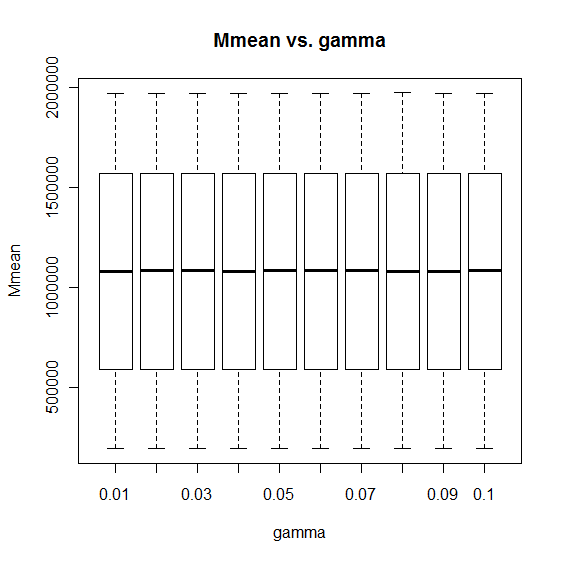
\includegraphics[height=6cm]{boxplot1000_mmean_gamma}
  % 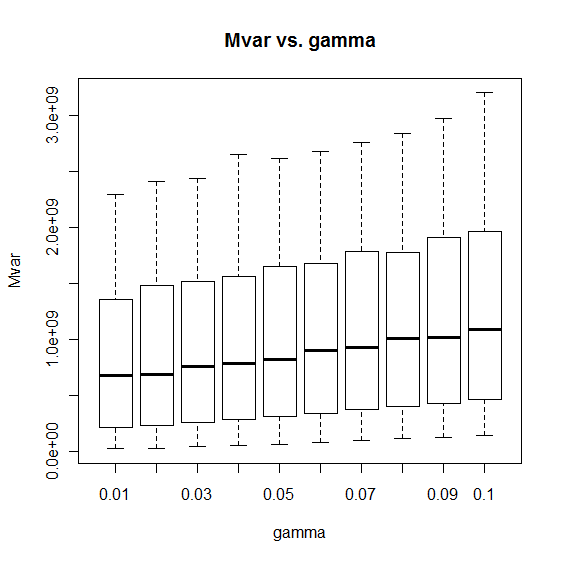
\includegraphics[height=6cm]{boxplot1000_mvar_gamma}
\end{frame}





\begin{frame}
  \frametitle{Results - M vs. P }
  \framesubtitle{500 iterations}
  \hspace*{-5mm}
  % 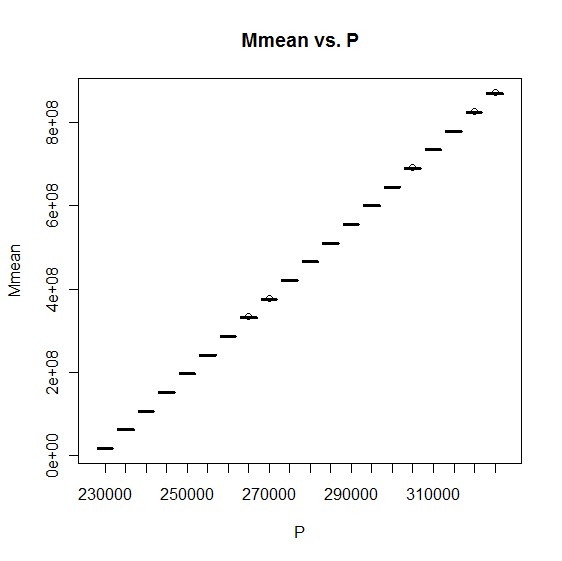
\includegraphics[height=6cm]{boxplot500_mmean_P}
  % 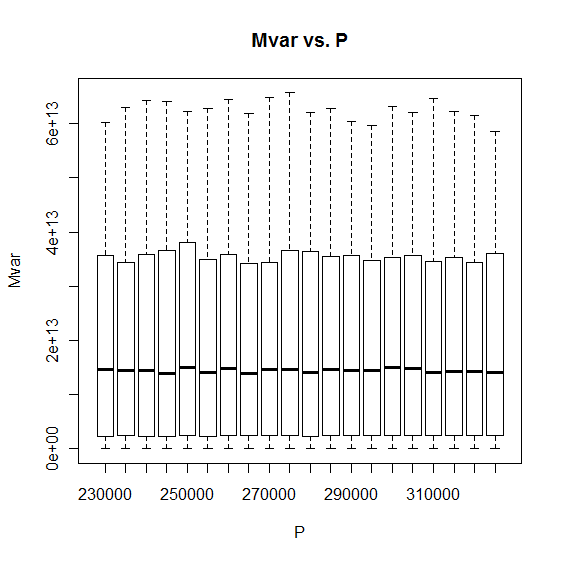
\includegraphics[height=6cm]{boxplot500_mvar_P}
\end{frame}


\begin{frame}
  \frametitle{Results - M vs. P }
  \framesubtitle{1000 iterations}
  \hspace*{-5mm}
  % 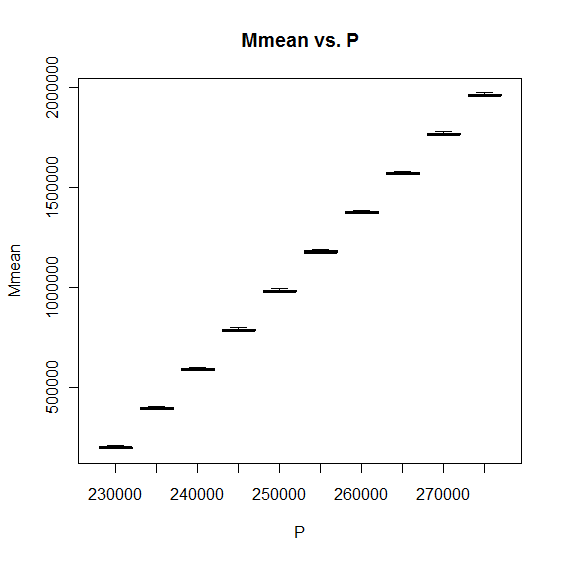
\includegraphics[height=6cm]{boxplot1000_mmean_P}
  % 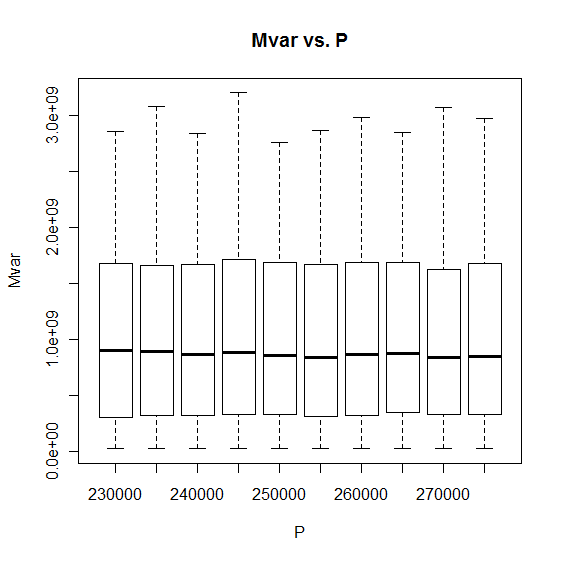
\includegraphics[height=6cm]{boxplot1000_mvar_P}
\end{frame}



\section{Conclusions}

\begin{frame}
  \frametitle{Conclusion}
  \begin{itemize}
  \item Stochastic Model of Deer-Collisions and Insurance Bond Funds 
  \item Consistent with basic benchmarks
  \item System most sensitive to $\alpha$
  \item Linear relationship between $M$ and $P$
  \item Initial $M$ may be too big
  \item Multivariate sensitivity should be examined
  \end{itemize}
\end{frame}







\section{Acknowledgments}

\begin{frame}
  \frametitle{Acknowledgments}
  Thanks to Dr. Joel Foisy, and NSF (NSF \# 1262737) for their
  support and involvement in this program.
\end{frame}



\end{document}
